\section{Einleitung}
\subsection{Motivation}
\begin{frame}
\frametitle{Motivation}
\vspace*{1cm}

\begin{itemize}
\item Große Anwendungsbreite von organischen Halbleitern
\item Polyacetylen als einfaches Testsystem
\item 1950-er \textsc{Longuet-Higgins}: Alternierende Bindungslängen
\item 1980-er \textsc{Su, Schrieffer, Heeger}: Anregungen (Soliton)
\end{itemize}
\vspace*{-.5cm}
\begin{center}
\hspace*{-4cm}\includegraphics[width = 14cm, angle = -20]{Images/polyacetylene/wavefunctions/HOMO_Side_View}
\end{center}
\end{frame}

\subsection{Dichtefunktionaltheorie}
\begin{frame}
\frametitle{Dichtefunktionaltheorie}
\begin{itemize}
\setlength{\itemsep}{.5cm}
\item Numerische, ab initio, Selbstkonsistenz-Methode zur Berechnung von quantenmechanischen Grundzuständen
\item \textsc{Hohenberg-Kohn}-Theorem: $\Psi \Rightarrow \rho$
\item \textsc{Kohn-Sham}-Orbitale $\varphi_i$ mit selber Elektronendichte
\begin{align*}
\rho(\vec{r}) &= \sum_i \left|\varphi_i\right|^2
\end{align*}
und Einteilchen-Hamiltonian:
\begin{align*}
\mathcal{H} &= \frac{\vec{p}^2}{2m} + V_\text{eff}(\vec{r}, \rho(\vec{r}))
\end{align*}
\item Unbekannte Terme in $V_\text{eff}(\vec{r}, \rho(\vec{r}))$: exchange-correlation-Term\\
Verwendete Approximation: PBE (GGA)
\end{itemize}
\end{frame}

\section{trans-Polyacetylen und SSH-Hamiltonian}
\subsection{trans-Polyacetylen}
\begin{frame}
\frametitle{\emph{trans}-Polyacetylen}
	\begin{figure}
		\parbox[b]{.6\linewidth}{\begin{tikzpicture}[show background rectangle]
\foreach \i in {0,2,4}{
	\draw (\i, 0) -- +(1,1);
	\draw (\i, 0.1) -- +(1,1);
	\draw (\i + 1, 1.05) -- +(1, -1);
	\draw (\i, 0) -- +(0,-.7) node[circle, fill = white, below] {H};
	\draw (\i + 1, 1) -- +(0,.7) node[circle, fill = white, above] {H};
	\node[circle, fill = white] (d\i) at (\i, 0) {C};
	\node[circle, fill = white] (u\i) at (\i + 1, 1) {C};
}
\draw [<->] (d0) -- (d2) node [midway, below] {$2a$};
\draw [->] (d2) -- +(.8, 0) node [below, yshift = -2] {$u$};
\draw [->] (d4) -- +(.8, 0) node [below, yshift = -2] {$u$};
\draw [->] (u2) -- +(-.8, 0) node [above, yshift = 2] {$u$};
\draw (6, 0) -- +(0,-.7) node[circle, fill = white, below] {H};
\node[circle, fill = white] (end) at (6,0) {C};
			\draw [dotted, line width = 1] (end) -- +(.5,.5);
			\draw [dotted, line width = 1] (d0) -- +(-.5,.5);
			\end{tikzpicture}}%
		\hspace{.04\linewidth}%
		\parbox[b]{.35\linewidth}{%
			\subcaption{Strukturformel: \emph{trans}-Polyacetylen}}
		\parbox[b]{.6\linewidth}{
			\begin{tikzpicture}[show background rectangle, xscale = .875, yscale = .7]
			\foreach \x in {0,...,6}{
				\draw[line width=1pt] (\x,0) .. controls (\x + 1, 2) and (\x - 1 , 2) .. cycle .. controls (\x + 1, -2) and (\x - 1 , -2) .. cycle;
			}
			\begin{scope}
			\clip (-.2, 2) rectangle (6.2, -2);
			\foreach \x in {0, 4}
			\foreach \y in {0, 1}
			\foreach \z in {-1, 1}
			\node at (\x + \y - \z + 1, \z) {\large +};
			\foreach \x in {0, 4}{
				\foreach \y in {0, 1}{
					\foreach \z in {-1, 1}{
						\node at (\x + \y - \z + 1, -\z) {\large -};
			}}}
			\end{scope}
			\draw[dotted, line width = 1] (-0.2,0) -- +(-.3,0);
			\draw[dotted, line width = 1] (6.2,0) -- +(.3,0);
			\end{tikzpicture}}%
		\hspace{.04\linewidth}%
		\parbox[b]{.35\linewidth}{%
			\subcaption{Schema: p-Orbitale von alternierende $\pi$-Bindung}}
	\end{figure}
\end{frame}


\subsection{Bindungslänge}
\begin{frame}
\frametitle{Bindungslänge}
\begin{minipage}{0.49\textwidth}
\begin{figure}[]
	\centering
	\includegraphics[width = .7\textwidth]{Images/polyacetylene/convergence/polyacetylene_nice_unit_cell}
	\captionsetup{justification = centering}
	\caption{Schema: Einheitszelle \emph{trans}-Polyacetylen}
\end{figure}
Berechnet: $a = \unit[1.23]{\AA}$\\
Literaturwert\footnotemark: $a = \unit[1.2]{\AA}$
\end{minipage}
\begin{minipage}{0.49\textwidth}
\begin{figure}
\centering
\includegraphics[width = .95\textwidth]{Images/polyacetylene/convergence/unit_cell_length}
\captionsetup{justification = centering}
\caption{Grundzustandsenergie in Abhängigkeit der Einheitszellenlänge}
\label{image_poly_cell_len}
\end{figure}
\end{minipage}
\footnotetext{{Alle Literaturwerte von: Su, Schrieffer, Heeger: Solitons in Polyacetylene. \& Kertesz, Choi, Yang: Conjugated Polymers and
Aromaticity.}}
\end{frame}

\subsection{Isooberflächen}
\begin{frame}
\frametitle{Isooberflächen am Rand der \textsc{Brillouin}-Zone}
\begin{figure}
\centering
\begin{subfigure}{0.4\textwidth}
\includegraphics[width = \textwidth]{Images/polyacetylene/wavefunctions/Homo_Cut}
\caption{HOMO-Band}
\label{image_homo1}
\end{subfigure}\hspace*{2cm}
\begin{subfigure}{0.4\textwidth}
\centering
\includegraphics[width = \textwidth]{Images/polyacetylene/wavefunctions/LUMO_Cut}
\caption{LUMO-Band}
\label{image_lumo1}
\end{subfigure}
\begin{subfigure}{\textwidth}
\centering
\includegraphics[width = 10cm]{Images/polyacetylene/wavefunctions/HOMO_Side_View}
\caption{Seitenansicht HOMO-Band}
\label{image_homo1_side_view}
\end{subfigure}
\end{figure}
\end{frame}

\begin{frame}
\frametitle{Verschiebung}
\begin{figure}
\centering
\centering
\includegraphics[width = \textwidth]{Images/polyacetylene/convergence/Potential_with_asymmetry}
\label{image_potential_with_asymmetry}
\caption{Grundzustandsenergie in Abhängigkeit von der Asymmetrie $\nicefrac{u}{u_0}$.}
\end{figure}
\begin{itemize}
\item Berechnung: $u = \unit[5\cdot10^{-3}]{\AA}$
\item Literaturwert: $u = \unit[0.042]{\AA}$
\end{itemize}
\end{frame}

\subsection{Tight-Binding Methode}
\begin{frame}
\frametitle{Tight-Binding Methode}
\begin{minipage}{0.49\textwidth}
	\begin{itemize}
	\setlength{\itemsep}{.5cm}
		\item Einteilchen-Methode
		\item Ausgangspunkt: Isolierte Atome\\
		ungestörte Wellenfunktionen
		\item Korrekturen $U$ durch Wechselwirkungen benachbarter Atome
		\item Bindender Zustand
		\begin{align*}
			\int\dd\vec{x}\ \varphi_1^*\cdot U\cdot \varphi_2&< 0
		\end{align*}
	\end{itemize}
\end{minipage}
\begin{minipage}{0.49\textwidth}
	\centering
	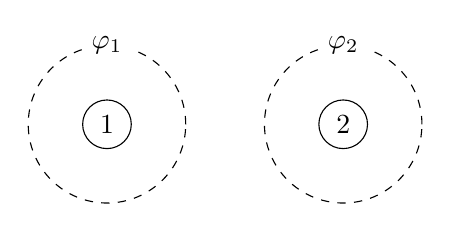
\begin{tikzpicture}
		\node [circle, draw] at (0,0) {1};
		\draw [dashed] (0,0) circle (1cm);
		\node [circle, draw] at (3,0) {2};
		\draw [dashed] (3,0) circle (1cm);
		\node [fill = white] at (0, 1) {$\varphi_1$};
		\node [fill = white] at (3, 1) {$\varphi_2$};
	\end{tikzpicture}
	\vspace*{1cm}
	
	\centering
	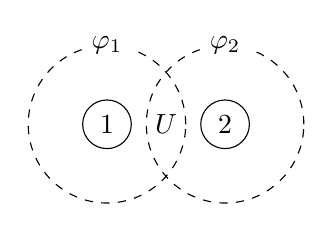
\begin{tikzpicture}
	\node [circle, draw] at (0,0) {1};
	\draw [dashed] (0,0) circle (1cm);
	\node [circle, draw] at (1.5,0) {2};
	\draw [dashed] (1.5,0) circle (1cm);
	\node [fill = white] at (0, 1) {$\varphi_1$};
	\node [fill = white] at (1.5, 1) {$\varphi_2$};
	\node at (0.75, 0) {$U$};
	\end{tikzpicture}
\end{minipage}
\end{frame}

\begin{frame}
\begin{minipage}{.39\textwidth}
	\begin{itemize}
		\setlength\itemsep{1cm}
		\item Polymer mit 'next-neighbour'-Interaktion
		\item Hamiltonian in der Basis der $\varphi_i$
		\item Positive Hopping-Parameter $t_i$
	\end{itemize}
\end{minipage}
\begin{minipage}{0.6\textwidth}
\centering
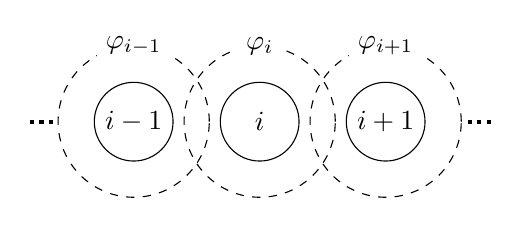
\begin{tikzpicture}[scale = .8]
	\foreach \i/\n in {0/i-1, 1/i, 2/i+1}{
		\node [circle, draw, minimum size = 1cm, inner sep = 0] at (2*\i, 0) {$\n$};
		\draw [dashed] (2*\i, 0) circle (1.2cm);
		\node [fill = white] at (2*\i, 1.2) {$\varphi_{\n}$};
	};
\draw [dotted, line width = 1.5] (-1.65, 0) -- +(.4, 0);
\draw [dotted, line width = 1.5] (5.3, 0) -- +(.4, 0);
\end{tikzpicture}
\\
\begin{align*}
\mathcal{H} &= \begin{pmatrix*}
\ddots&&&\\
&E_{0}&-t_{i-1, i}&0\\
&-t_{i, i-1}&E_0&-t_{i, i+1}\\
&0&-t_{i+1, i}&E_{0}&\\
&&&&\ddots
\end{pmatrix*}
\end{align*}
\\
\begin{align*}
	\mathcal{H} &= \sum_i E_0 n_i - \sum_i t_{i, i+1} \left(c_i^\dagger\  c_{i+1} + c_{i+1}^\dagger\  c_i\right)
\end{align*}
\end{minipage}
\end{frame}

\subsection{trans-Polyacetylen und SSH-Hamiltonian}
\begin{frame}
\frametitle{SSH-Hamiltonian}
\centering
\begin{tikzpicture}[show background rectangle, yscale = .7]
\foreach \i in {0,2,4}{
	\draw (\i, 0) -- +(1,1);
	\draw (\i, 0.1) -- +(1,1);
	\draw (\i + 1, 1.05) -- +(1, -1);
	\draw (\i, 0) -- +(0,-.7) node[circle, fill = white, below] {H};
	\draw (\i + 1, 1) -- +(0,.7) node[circle, fill = white, above] {H};
	\node[circle, fill = white] (d\i) at (\i, 0) {C};
	\node[circle, fill = white] (u\i) at (\i + 1, 1) {C};
}
\draw [<->] (d0) -- (d2) node [midway, below] {$2a$};
\draw [->] (d2) -- +(.8, 0) node [below, xshift = 6, yshift = -2] {$u_{n-1}$};
\draw [->] (d4) -- +(.8, 0) node [below, xshift = 6, yshift = -2] {$u_{n+1}$};
\draw [->] (u2) -- +(-.8, 0) node [above, yshift = 2] {$u_{n}$};
\draw (6, 0) -- +(0,-.7) node[circle, fill = white, below] {H};
\node[circle, fill = white] (end) at (6,0) {C};
\draw [dotted] (end) -- +(.5,.5);
\draw [dotted] (d0) -- +(-.5,.5);
\end{tikzpicture}
\vspace*{1cm}

\scalebox{.9}{\parbox{\textwidth}{
\begin{align*}
\mathcal{H}_\text{SSH} &= \underbrace{-2\sum_{n} t_{n+1,n}\left(c_{n+1}^\dagger c_n + c_n^\dagger c_{n+1}\right)}_{\text{Elektronen Hopping / $\pi$-Bindungsenergie}}\quad +\underbrace{\frac{1}{2}\sum_n \kappa (u_{n+1} - u_n)^2}_{\sigma-\text{Bindungsenergie}} + \underbrace{\frac{1}{2} \sum_n M \dot{u}^2_n}_{\text{Kinetische Energie}}
\end{align*}
}}
\end{frame}

\subsection{\textsc{Peierls}-Instabilität}
\begin{frame}
\frametitle{\textsc{Peierls}-Instabilität}
\centering
\begin{tikzpicture}[show background rectangle, scale = .9]
\pgfmathsetmacro{\j}{0.5};
\draw (0,0) -- (6,0);
\foreach \i in {0,2,...,6}{
	\draw[fill = black] ({\i + \j * (-1)^(\i/2)},0) circle (0.1);
	\draw[] (\i,-0.1) -- (\i, 0.1);
}
\draw[<->] (2 - \j, -1) -- (6 - \j, -1) node[midway, fill = white] {2a};
\draw[<->] (0 + \j, -0.5) -- (4 + \j, -0.5) node[midway, fill = white] {2a};
\draw[<->] (2 - \j, 0.5) -- (2, 0.5) node[midway, above] {$u$};
\draw[<->] (4, 0.5) -- (4 + \j, 0.5) node[midway, above] {$u$};
\draw[dotted] (-0.3,0) -- (6.3, 0);
\end{tikzpicture}
\begin{itemize}
	\item \textsc{Peierls}-Instabilität $\to$ $u_n = (-1)^nu$
	\item Halbe \textsc{Brillouin}-Zone
	\item Hopping-Hamiltonian:
	\begin{align*}
		\mathcal{H}_\text{hopp} &= -2\sum_n \left[t_0 + (-1)^n\delta\right]\cdot\left(c_{n+1}^\dagger c_n + c_n^\dagger c_{n+1}\right)
	\end{align*}
	mit $\delta = 2\alpha u$\\
	und Phonon-Kopplungs-Konstante:
	\begin{align*}
		\alpha = \nicefrac{\partial t}{\partial u}
	\end{align*}
\end{itemize}
\end{frame}

\subsection{Bandstruktur}
\begin{frame}
\frametitle{Bandstruktur}
\begin{figure}
	\centering
	\vspace*{-.5cm}
	\begin{subfigure}{0.49\textwidth}
		\includegraphics[width =\textwidth]{Images/Plots/bandstructure_without_gap}
		\caption{Bandstruktur für $u = 0$.}
		\label{image_bs_wo_gap}
	\end{subfigure}\hspace*{0.2cm}
	\begin{subfigure}{0.49\textwidth}
		\includegraphics[width = \textwidth]{Images/Plots/bandstructure_with_gap}
		\caption{Bandstruktur für $u \neq 0$.}
		\label{image_bs_w_gap}
	\end{subfigure}
\end{figure}
\begin{align*}
	E_k = \pm \sqrt{\left(\smash[b]{\underbrace{2t_0\cos(ka)}_{=:\epsilon_k}}\right)^2 + \left(\smash[b]{\underbrace{2\delta\sin(ka)}_{=:\Delta_k}}\right)^2}
\end{align*}
\end{frame}